\section{Additional Analyses of Behavioral Rate}

\subsection{Weight Reconstruction Does Not Predict Behavior}
\begin{table}[t]
\caption{Candidates that do not determine $R^\star(0.90)$. 81 adapters over five corpora (MetaMathQA, Magicoder, XSum, hh-rlhf, Alpaca) on Mistral-7B and Qwen2.5-7B, NF4, rank 16, 8k rows, 4 epochs, 3 seeds; plus the 268-cell rate-law audit over four receivers (Appendix~\ref{app:xp_details}).}
\label{tab:not-rstar}
\centering
\small
\begin{tabular}{p{0.34\linewidth}p{0.58\linewidth}}
\toprule
candidate & result \\
\midrule
distinct rows & ranks 4 correctly inside a corpus, backwards across corpora \\
behavioural change (bits saved) & slope 1.90 inside a 0.16-wide window; 0.12 on answer rewrites, flat on optimizer budget \\
optimizer depth & 16$\times$ the updates on the same rows moves bits saved by 0.04 and $R^\star$ down \\
base surprisal on the corpus & $r=+0.25$ with $R^\star$ \\
weight reconstruction error & constant to about 1\% across all five corpora at a fixed rate \\
local curvature ($g^\top\delta$, $\tfrac12\delta^\top H\delta$) & second order adds no ranking power; the expansion fails below 1 bit per value \\
\bottomrule
\end{tabular}
\end{table}

\subsection{Equal Bit Budgets Are Not Functionally Interchangeable}
\label{app:layer-location}

The previous experiment shows that the magnitude of a compression error is
not sufficient to predict its behavioral cost. We next ask whether its
location matters. We compare uniform precision with matched-rate variants in
which precision is reduced preferentially in the early, middle, or late third
of the transformer.
\newline
Figure~\ref{fig:layer-location} shows that uniform allocation preserves more
fine-tuning gain at both 0.5 and 1.0 bits per value, while reducing precision
in the final third is most damaging. This is not explained by larger updates
in later layers: weight-update RMS is approximately flat across depth, whereas
the induced hidden-state shift grows toward the final layers.
\newline
Together with the RMSE counterexample, this shows that adapter compression is
functionally non-uniform: neither total parameter error nor total bit budget
determines behavioral distortion on its own. 

\begin{figure}[t]
\centering
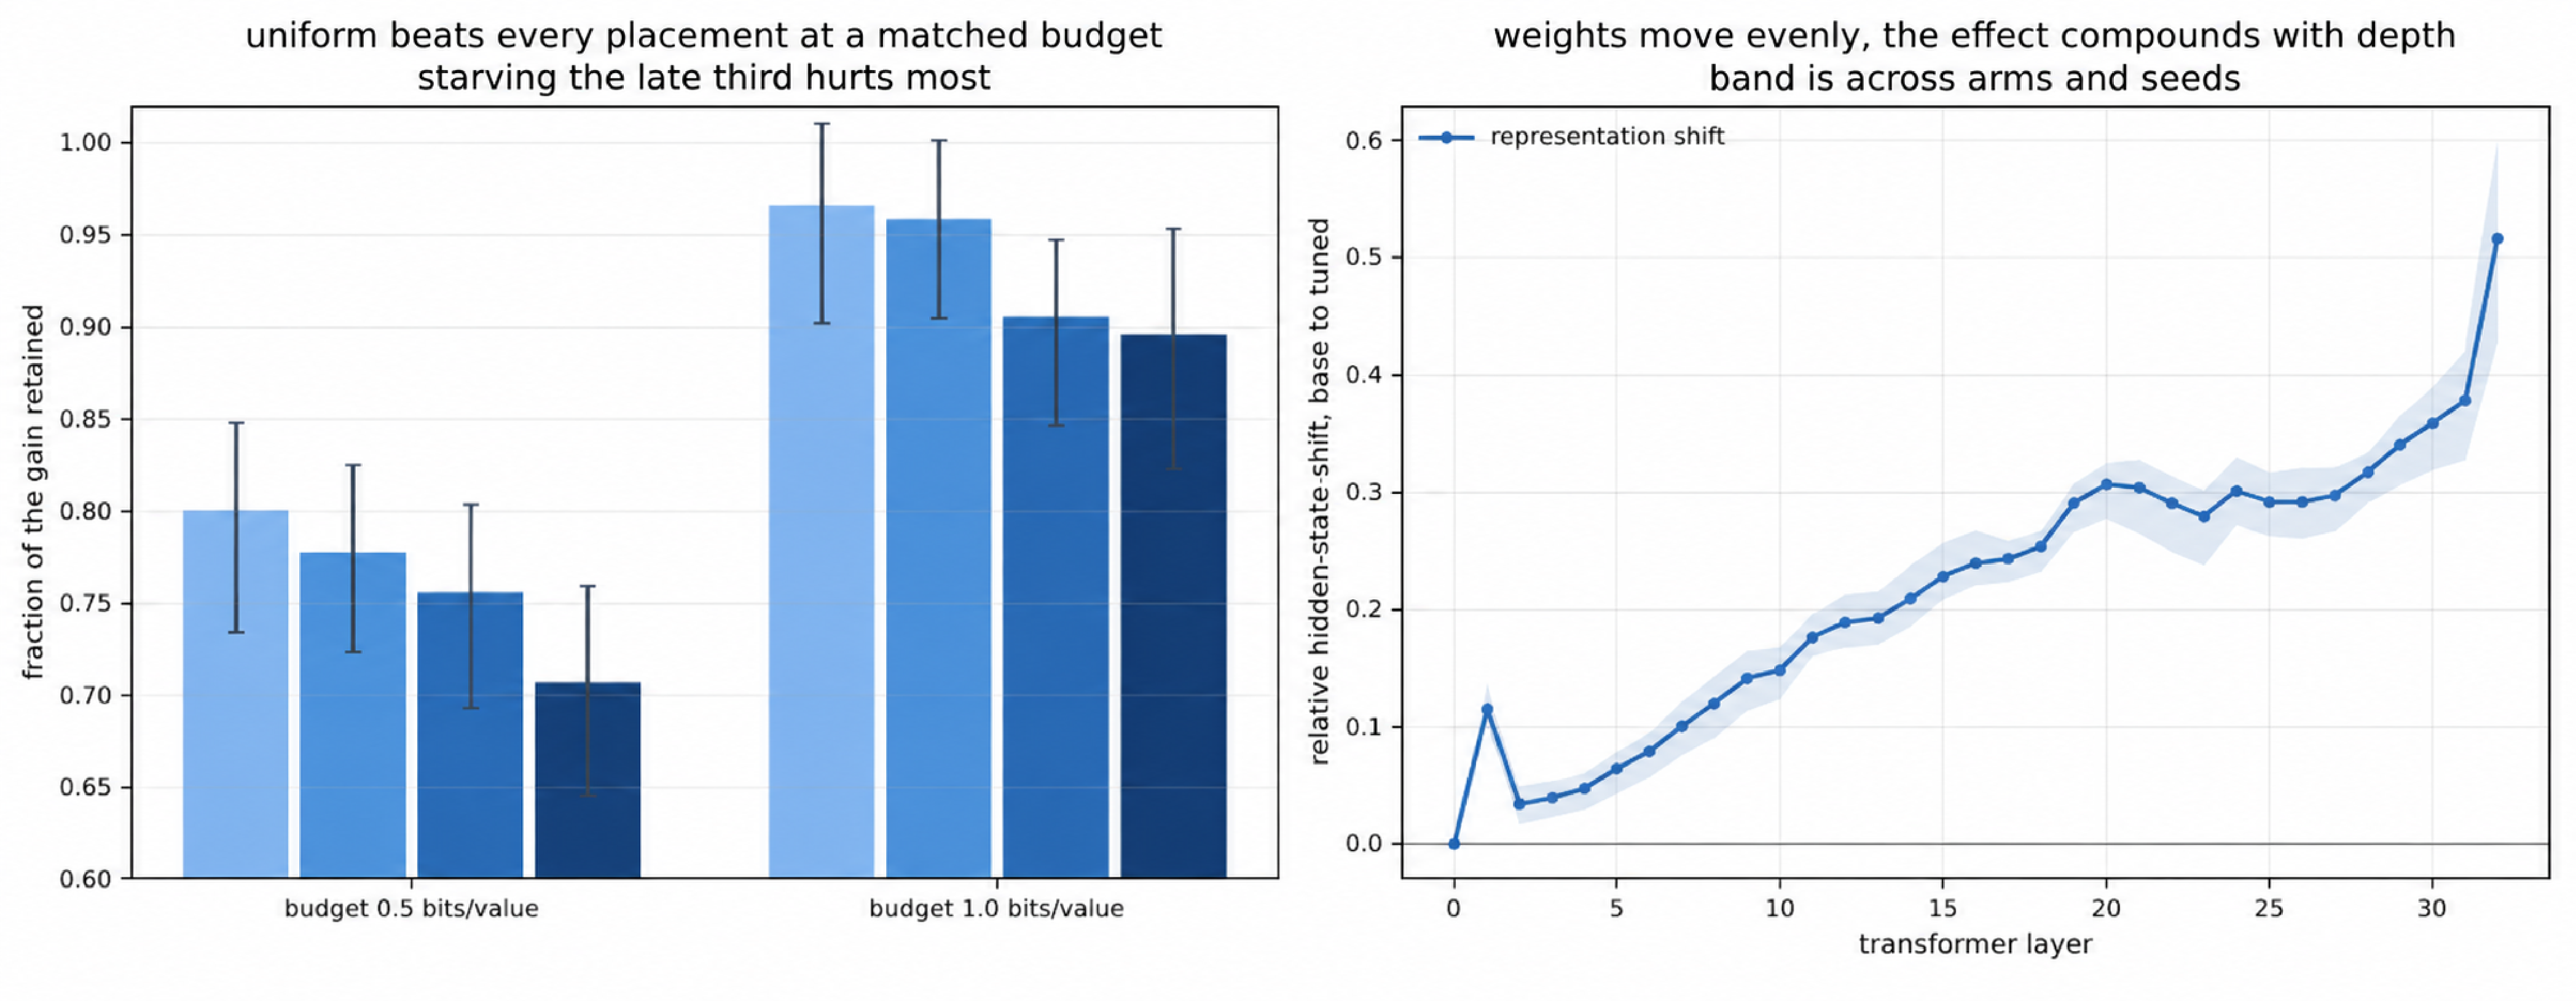
\includegraphics[width=0.8\linewidth]{figures/F4_layer_location.pdf}
\caption{
\textbf{Equal bit budgets are not functionally interchangeable.}
Left: retained gain under uniform or depth-selective compression at matched
budgets. Right: hidden-state shift grows with depth despite approximately
flat update magnitude.
}
\label{fig:layer-location}
\end{figure}

\subsection{The Rate Across Receivers}

\begin{figure}[h]
\centering
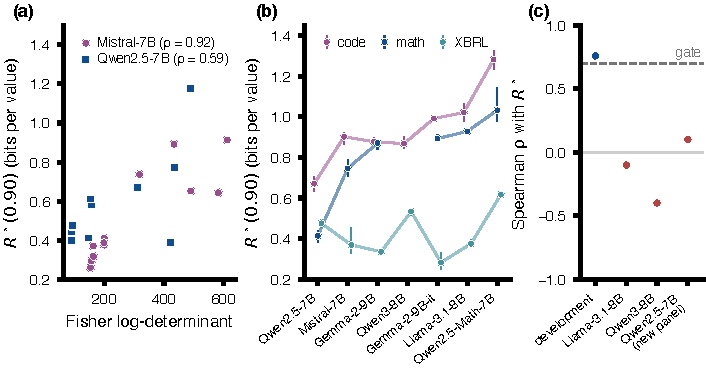
\includegraphics[width=0.8\linewidth]{figures/F10_predictor.pdf}
\caption{The rate belongs to the dataset--receiver pair. (a) Correction-spectrum log-determinant against $R^\star(0.90)$, one point per arm, within the two development receivers. (b) $R^\star(0.90)$ of three corpora on seven receivers; bars span seeds. The ordering of corpora changes with the receiver.}
\label{fig:predictor}
\end{figure}

\subsection{Recovery controls}

\begin{table}[h]
\caption{Accuracy (\%) on GSM8K (1,319) and GSM-Symbolic (500, clustered by template), means of 3 seeds. Frozen base: 77.56 / 71.40. The random rank-1 projection also reaches the base, so direction choice alone does not explain the recovery.}
\label{tab:ladder}
\centering
\small
\begin{tabular}{lrr}
\toprule
condition & GSM8K & GSM-Symbolic \\
\midrule
rank 1 @ 1 bit & \textbf{83.24} & \textbf{77.60} \\
rank 1 @ 16 bits & 42.81 & 33.80 \\
full rank @ 1 bit & 65.05 & 55.00 \\
full rank @ 16 bits (damaged) & 23.81 & 15.53 \\
random rank-1 projection @ 16 bits & 80.09 & 72.13 \\
full update scaled to the rank-1 norm & 23.93 & 13.80 \\
residual rank 15 @ 16 bits & 30.86 & 25.20 \\
\bottomrule
\end{tabular}
\end{table}
% GSM8K 1,319 problems; GSM-Symbolic 500, intervals clustered by template. Qwen2.5-7B, 3 seeds.
